\documentclass[12pt, twoside]{article}
% \documentclass[12pt, twoside]{article}
\usepackage[letterpaper, margin=1in, headsep=0.2in]{geometry}
\setlength{\headheight}{0.6in}
%\usepackage[english]{babel}
\usepackage[utf8]{inputenc}
\usepackage{microtype}
\usepackage{amsmath}
\usepackage{amssymb}
%\usepackage{amsfonts}
\usepackage[nomessages]{fp} %\FPeval{\var-name}{2*sin(pi/6)}
\usepackage{siunitx} %units in math. eg 20\milli\meter
\usepackage{yhmath} % for arcs, overparenth command
\usepackage{tikz} %graphics
\usetikzlibrary{quotes, angles, arrows, arrows.meta}
\usepackage{graphicx} %consider setting \graphicspath{{images/}}
\usepackage{parskip} %no paragraph indent
\usepackage{enumitem}
\usepackage{multicol}
\usepackage{venndiagram}

\usepackage{fancyhdr}
\pagestyle{fancy}
\fancyhf{}
\renewcommand{\headrulewidth}{0pt} % disable the underline of the header
\raggedbottom
\hfuzz=2mm %suppresses overfull box warnings

\usepackage{hyperref}
\usepackage{float}

\fancyhead[LE]{\thepage}
\fancyhead[RO]{\thepage \\ First and last name: \hspace{2.5cm} \,\\ Section: \hspace{2.5cm} \,}
\fancyhead[LO]{BECA/Huson/Geometry: Construction \\* 25 October 2024}

\begin{document}
\subsubsection*{2.7 Test: Solving for length and angle measures}
\begin{enumerate}[itemsep=0.5cm]
  \item Two points $A(-1)$, $B(3)$ and the segment $\overline{AB}$ are shown on the number line. \par \smallskip
    \begin{tikzpicture}
      \draw [<->] (-2.5,0)--(4.5,0);
      \draw [-, thick] (-1,0)--(3,0);
      \foreach \x in {-2,...,4} %2 leading for diff!=1
      \draw[shift={(\x,0)},color=black] (0pt,-3pt) -- (0pt,3pt) node[below=5pt]  {$\x$};
      \draw [fill] (-1,0) circle [radius=0.05] node[above] {$A$};
      \draw [fill] (3,0) circle [radius=0.05] node[above] {$B$};
    \end{tikzpicture} \par \smallskip
    What is the length of the segment $\overline{AB}$? Show your work as an equation. \vspace{2cm}
  
\item Given $\overline{PQR}$, $PQ=7 \frac{1}{4}$, and $QR=3 \frac{3}{4}$. Find ${PR}$.\par  \vspace{0.5cm}
  \begin{tikzpicture}
    \draw [-, thick] (1,0)--(7,0);
    \draw [fill] (1,0) circle [radius=0.05] node[below]{$P$};
    \draw [fill] (5,0) circle [radius=0.05] node[below]{$Q$};
    \draw [fill] (7,0) circle [radius=0.05] node[below]{$R$};
  \end{tikzpicture}  \vspace{2cm}

\item Given $\overline{DEF}$, $DE=x+6$, $EF=4x+7$, $DF=18$. Find ${DE}$.\vspace{1cm}
  \begin{center}
    \begin{tikzpicture}
        \draw [-, thick] (0,0)--(8,0);
        \draw [fill] (0,0) circle [radius=0.05] node[below]{$D$};
        \draw [fill] (3,0) circle [radius=0.05] node[below]{$E$};
        \draw [fill] (8,0) circle [radius=0.05] node[below]{$F$};
    \end{tikzpicture}
  \end{center}


\newpage
\item Apply the Angle Addition postulate. Write and equation to support your work.
\begin{multicols}{2}
  Given m$\angle ABD = 80^\circ$ and \\[0.25cm] m$\angle DBC = 20^\circ$. \\[0.5cm]
  Find $m \angle ABC$. \\
  \begin{tikzpicture}[scale=1.4]
    \draw[<->, thick]
      (3,0) coordinate (a) node[below left] {$C$}
      -- (0,0) coordinate (b) node[below left] {$B$}
      -- (2,1.5) coordinate (c) node[below right] {$D$}
      pic["$20^\circ$", <->, draw=black, angle eccentricity=1.5, angle radius=1cm]
      {angle=a--b--c};
      \draw[<-, thick]
      (-1,2) coordinate (d) node[right] {$A$}
      -- (0,0) coordinate (e)
      pic["$80^\circ$", <->, draw=black, angle eccentricity=1.25, angle radius=1cm]
      {angle=c--e--d};
  \end{tikzpicture}
\end{multicols}

\item Given the angle measures and situation shown, write an equation and solve for $x$.
  \begin{multicols}{2}
    m$\angle ABD = 5x$ \\[0.25cm]
    m$\angle DBC = 45^\circ$ \\[0.25cm]
    $m \angle ABC = 145^\circ$ \\
    \begin{tikzpicture}[scale=2]
      \draw[<->, thick]
        (-20:2) coordinate (a) node[below left] {$C$}
        -- (0,0) coordinate (b) node[below left] {$B$}
        -- (20:3) coordinate (c) node[below right] {$D$}
        pic["$45^\circ$", <->, draw=black, angle eccentricity=1.5, angle radius=1cm]
        {angle=a--b--c};
        \draw[<-, thick]
        (110:1.5) coordinate (d) node[right] {$A$}
        -- (0,0) coordinate (e)
        pic["$5x$", <->, draw=black, angle eccentricity=1.5, angle radius=1cm]
        {angle=c--e--d};
    \end{tikzpicture}
  \end{multicols} \vspace{1cm}

\item Two lines intersect with m$\angle 1=80^\circ$ and m$\angle 3=4x$. Find $x$.\bigskip
  \begin{flushleft}
  \begin{tikzpicture}[scale=0.6]
    \draw[<->, thick] (0,-1.5)--(10,1.5);
    \draw[<->, thick] (2,3.5)--(7,-3.5);
    \node at (2,.4){m$\angle 1=80^\circ$};
    \node at (7,-.6){m$\angle 3=4x$};
    \node at (5,1){2};
    \node at (4,-1){4};
  \end{tikzpicture}
  \end{flushleft}

\newpage
\item Given the angle measures and perpendicular situation shown, $\overrightarrow{BD} \perp \overleftrightarrow{ABC}$. Find $x$. \vspace{0.2cm}
\begin{multicols}{2}
  m$\angle DBE =3x+20^\circ$ \\[0.25cm]
  m$\angle EBC = 6x -2^\circ$ \\[0.25cm]
  \begin{tikzpicture}[scale=1]
    \draw[<->, thick]
      (0:4) coordinate (a) node[below left] {$C$}
      -- (0,0) coordinate (b) node[below] {$B$}
      -- (50:4) coordinate (c) node[below right] {$E$}
      pic["$6x -2$", <->, draw=black, angle eccentricity=2, angle radius=1cm]
      {angle=a--b--c};
      \draw[<-, thick]
      (90:3) coordinate (d) node[right] {$D$}
      -- (0,0) coordinate (e)
      pic["$3x+20^\circ$", <->, draw=black, angle eccentricity=1.5, angle radius=1.5cm]
      {angle=c--e--d};
      \draw[->, thick] (0,0)--(-180:2) node[below right]{$A$};
      \draw (0,0)++(-0.3,0)--++(0,0.3)--+(0.3,0);
  \end{tikzpicture}
\end{multicols} \vspace{1cm}

\item A linear pair have measures m$\angle ABD = 10x + 28^\circ$ and m$\angle DBC = 12x -2^\circ$. \\[0.2cm] 
Find m$\angle ABD$. Check your answer. \vspace{0.5cm}
\begin{flushright}
  \begin{tikzpicture}[scale=1.2]
    \draw[<->, thick]
      (0:3) coordinate (a) node[below left] {$C$}
      -- (0,0) coordinate (b) node[below] {$B$}
      -- (75:3) coordinate (c) node[below right] {$D$}
      pic["$12x -2$", <->, draw=black, angle eccentricity=2, angle radius=1cm]
      {angle=a--b--c};
      \draw[<-, thick]
      (180:3) coordinate (d) node[below] {$A$}
      -- (0,0) coordinate (e)
      pic["$10x + 28$", <->, draw=black, angle eccentricity=1.5, angle radius=1cm]
      {angle=c--e--d};
      %\draw[->, thick] (0,0)--(-180:2) node[below right]{$A$};
      %\draw (0,0)++(-0.3,0)--++(0,0.3)--+(0.3,0);
  \end{tikzpicture}
\end{flushright} \vspace{5cm}

\item Triangle $ABC$ has angle measures $m\angle A = 45^\circ$, $m\angle B = 60^\circ$. Find the measure of the third angle, $m\angle C$.\vspace{1cm}

\newpage
\item Construct an equilateral triangle with one side $\overline{AB}$.  
  \vspace{5cm}
  \begin{center}
  \begin{tikzpicture}
    \draw [-, thick] (0,0)--(5,1);
    \draw [fill] (0,0) circle [radius=0.05] node[below]{$A$};
    \draw [fill] (5,1) circle [radius=0.05] node[below]{$B$};
  \end{tikzpicture}
  \end{center}

\item Construct an angle bisector of the given angle.
  \vspace{3cm}
  \begin{center}
  \begin{tikzpicture}
    \draw [<->, thick] (-7,2)--(0,0)--(0.5,7);
    %\draw [fill] (0,0) circle [radius=0.05] node[below]{$A$};
  \end{tikzpicture}
  \end{center} \vspace{1cm}

\newpage
\item Construct a perpendicular bisector of $\overline{PQ}$.  
  \vspace{4cm}
  \begin{center}
  \begin{tikzpicture}
    \draw [-, thick] (0,0)--(5,-2);
    \draw [fill] (0,0) circle [radius=0.05] node[below]{$P$};
    \draw [fill] (5,-2) circle [radius=0.05] node[below]{$Q$};
  \end{tikzpicture}
  \end{center} 
  \vspace{3cm}

\item Construct a perpendicular to line $l$ through the point $P$.  
    \vspace{3cm}
    \begin{center}
    \begin{tikzpicture}
        \draw [<->, thick] (0,0)--(10,-5) node [below right]{$l$};
        \draw [fill] (4,-2) circle [radius=0.05] node[below left]{$P$};
    \end{tikzpicture}
    \end{center}

\newpage
\item Translate $\triangle ABC$ right six and down two units. Label the image $\triangle A'B'C'$.
\begin{center}
    \begin{tikzpicture}[scale=0.7]
    \draw [help lines] (-8,-6) grid (8,6);
    \draw [thick, <->] (-8.4,0) -- (8.4,0) node [right] {$x$};
    \draw [thick, <->] (0,-6.4)--(0,6.4) node [above] {$y$};  
    \draw [thick]
      (-1,4) node[above right] {$A$}--
      (-4,-1) node[below] {$B$}--
      (-1,-1) node[below right] {$C$}--cycle;  
  \end{tikzpicture}
\end{center}

\item Reflect $\triangle DEF$ across the $y$-axis, labeling the image $\triangle D'E'F'$.
\begin{center}
    \begin{tikzpicture}[scale=.7]
    \draw [help lines] (-8,-6) grid (8,6);
    \draw [thick, <->] (-8.4,0) -- (8.4,0) node [right] {$x$};
    \draw [thick, <->] (0,-6.4)--(0,6.4) node [above] {$y$};  
    \draw [thick]
      (-2,-4) node[above right] {$D$}--
      (-5,-1) node[above right] {$E$}--
      (-7,-3) node[below left] {$F$}--cycle;  
  \end{tikzpicture}
\end{center}

\newpage
\item Rotate the triangle $90^\circ$ counterclockwise around the origin, $\triangle ABC \rightarrow \triangle A'B'C'$. Complete the table of the coordinates and plot and label the image on the grid. \vspace{0.5cm}
\begin{multicols}{2}
  $A(0,0) \rightarrow$ \\[0.7cm]
  $B(3,2) \rightarrow$ \\[0.7cm]
  $C(3,0) \rightarrow$ \\[0.7cm]
    \begin{tikzpicture}[scale=.70]
    \draw [help lines] (-5,-5) grid (5,5);
    \draw [thick, <->] (-5.4,0) -- (5.4,0) node [right] {$x$};
    \draw [thick, <->] (0,-5.4)--(0,5.4) node [above] {$y$};  
    \draw [thick]
      (0,0) node[below left] {$A$}--
      (3,2) node[above right] {$B$}--
      (3,0) node[below right] {$C$}--cycle;  
    \end{tikzpicture}
  \end{multicols}

\item A reflection maps $P(7,-3)$ onto $P'(7,3)$. Is the reflection across the $x$-axis or the $y$-axis? \vspace{2cm}

\item Specify the translation that maps $Q(11,-2)\rightarrow Q'(6,7)$. \vspace{2cm}

\item Triangle $X'Y'Z'$ is the image of triangle $XYZ$ after a translation. Which triangle is larger, or are they the same size? Justify your answer. \vspace{3cm}


\newpage
\item Simplify each expression by combining like terms. (exact answers only, no decimals)
  \begin{multicols}{2}
      \begin{enumerate}[itemsep=1.5cm]
        \item $6x+4-3x+2$
        \item $-3y^2-5y+7y+2y^2$
        \item $4+6\pi+8-2\pi$
        \item $10x-6x+3\sqrt{7}+4\sqrt{7}$
      \end{enumerate}
  \end{multicols} \vspace{1cm}

\item Use the function $f(x) = \frac{1}{2}x+5$ to answer the questions.
  \begin{multicols}{2}
  \begin{enumerate}[itemsep=2cm]
      \item What is $f(0)$?
      \item Find $f(-2)$
      \item What is $x$ when $f(x) = 15$?
  \end{enumerate}
  \end{multicols} \vspace{2cm}

\item Solve each equation for $x$. Then check your answer.
  \begin{multicols}{2}
    \begin{enumerate}[itemsep=1cm]
  \item $3x + 4x - 15 = 34$
  \item $6x - 9 = 7x - 12$
  \end{enumerate}
  \end{multicols}


\end{enumerate}
\end{document}